\documentclass[10pt,a4paper]{article}
\usepackage[utf8]{inputenc}
\usepackage[margin=1.2cm,includehead,includefoot]{geometry}
\usepackage[default]{lato}
\usepackage[T1]{fontenc}
\usepackage{multicol}
\usepackage{fancyhdr}
\usepackage{titlesec}
\usepackage{graphicx}
\usepackage{pdfpages}

\titlespacing{\subsection}{0em}{-0.1em}{-1.25em}
\titlespacing{\section}{0em}{0em}{0em}

%\titleformat{name=\subsection}
%{\normalfont\bfseries}{\thesubsection}{-1.25em}{}{}

\usepackage{url}
\usepackage{breakurl}
\def\UrlBreaks{\do\/\do-}

\usepackage{enumitem}
\setitemize{noitemsep,topsep=0pt,parsep=0pt,partopsep=0pt}
\setenumerate{noitemsep,topsep=0pt,parsep=0pt,partopsep=0pt}

\titleformat{\section}{\normalfont\Large\bfseries}{}{0em}{}
\titleformat{\subsection}{\normalfont\bfseries}{}{0em}{}

\pagestyle{fancy}
\fancyhf{}
\fancyhead[R]{\leftmark}
\fancyhead[L]{The Librarian}
\fancyfoot[C]{\thepage}

\renewcommand{\footrulewidth}{0.5pt}
\setlength{\headsep}{1.5em}

\setlength{\parindent}{0em}
\setlength{\parskip}{1.25em}

\newcounter{count}

\begin{document}

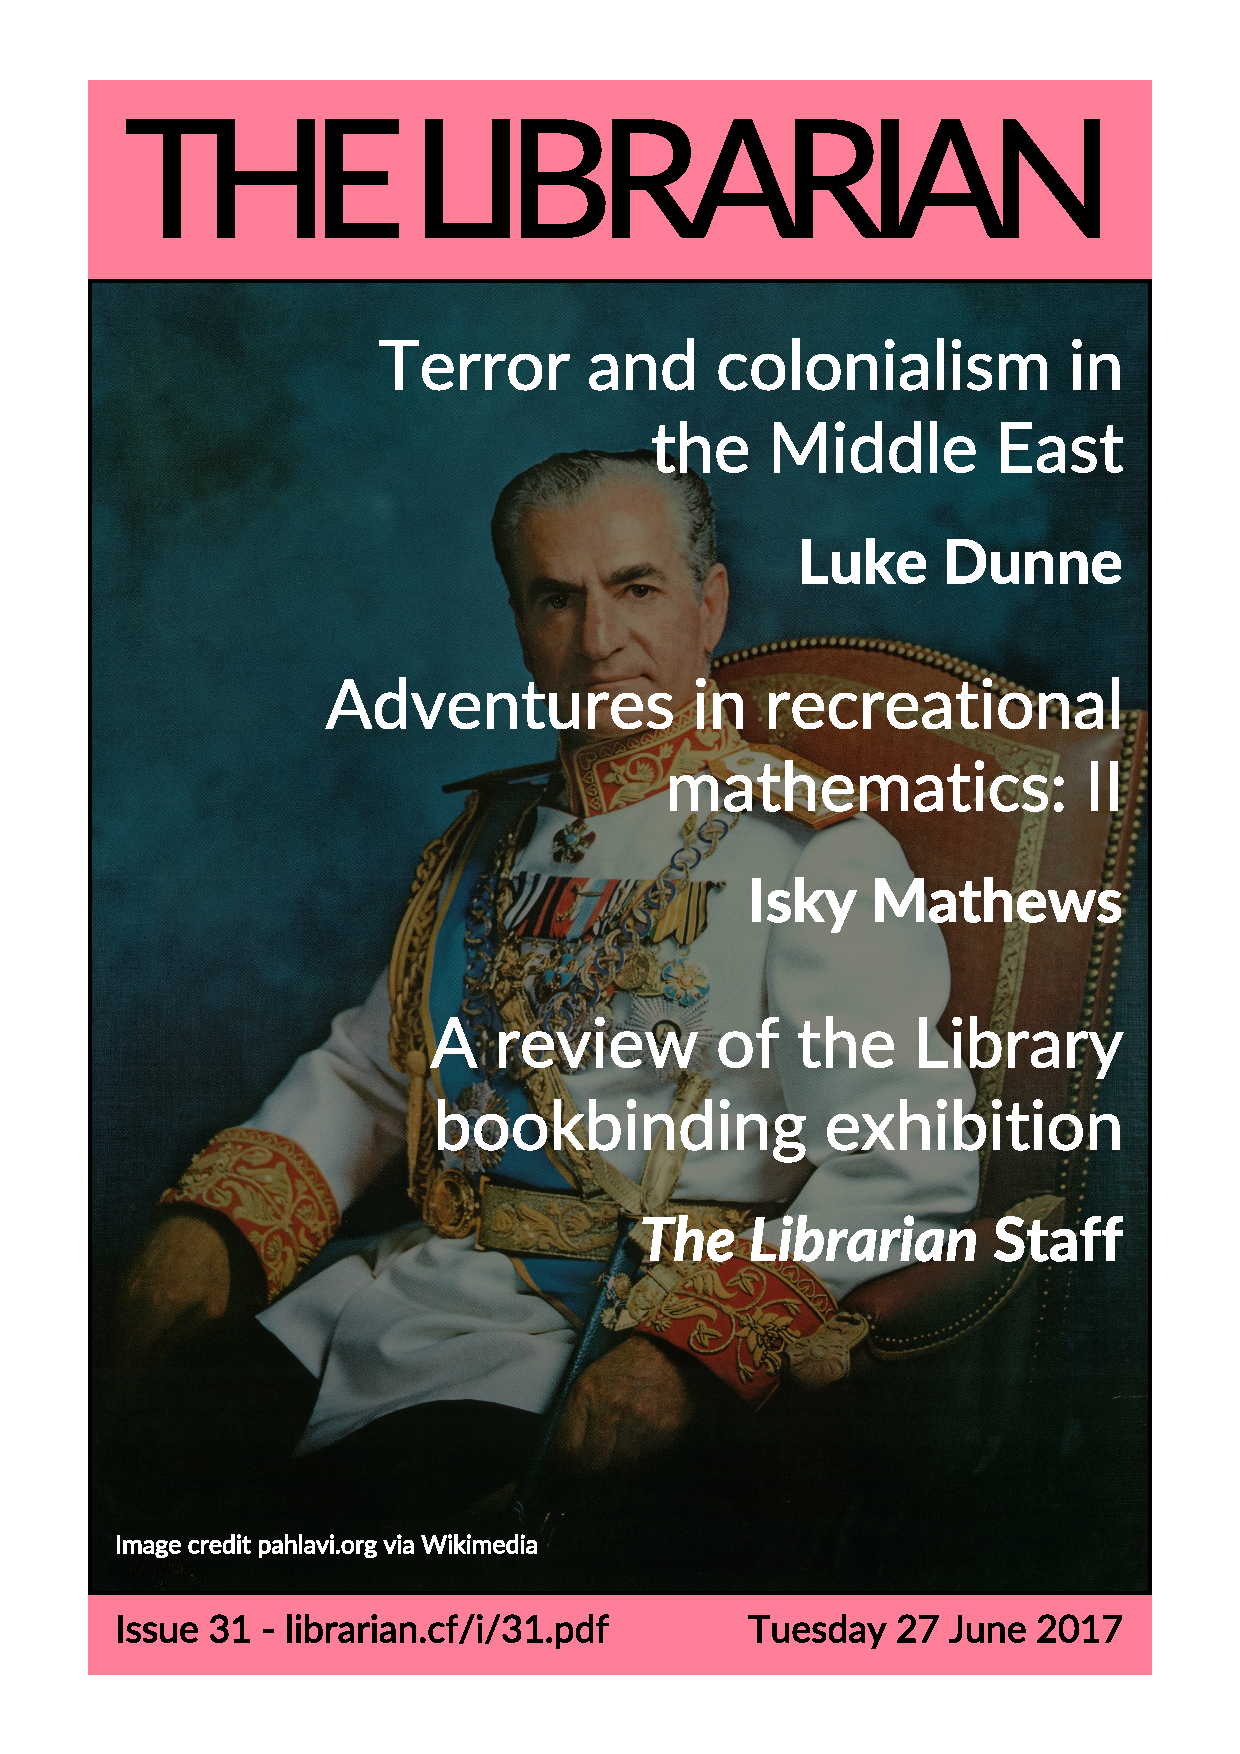
\includepdf[pages={1}]{cover.pdf}

\section{Library News}

\textbf{Compiled by Jonny Heywood, Chairperson, and edited by Joshua Loo}

\begin{multicols}{2}

\subsection{Bookbinding comes to the Library}

This month the school bookbinders set up their annual bookbinding exhibition up Library which is still on display in the Brock Room. Featuring dozens of items, from novels and notebooks to delicately decorated symbols and letters, the display celebrates the highlights of a year’s diligent binding in Weston’s basement as well as introducing passers-by in the library to what one binder called the ‘art of the bind’. Highlights include Dominic Brind’s binding of a book on Charles V with a “golden fleece”, Captain Emeritus of Debating, Senior Binder Alfred Murray’s binding of Vita Nuova with ethereal angels on a navy leather backdrop, and the Dean's Presentation Binding, in the style of formal abbey dress, the first of Westminster's unique "cassock bindings", also Alfred Murray’s work. 

On one visit, Alfred was there totting up numbers of books bound by each house (as I left it, Dryden’s led Purcell’s, then College), calculating who would win the annual ‘House Bookbinding Competition’, the winner being the house which has bound the most books since the start of the year. Alfred is the Head Bookbinder, and has an imposing collection of books on display numbering more than any other student, representing an impressive juggling act with A-Levels. 

Benedict Randall Shaw, long-time contributor to the Librarian, and avid bookbinder, when asked about bookbinding, replied that “It’s a very complex process. To put it simply, one first splits the book into its composite sections, before sewing them onto cords or tape, and often rounding them for aesthetic purposes. One then sews a 'headband' on, and puts boards on the ends of the book, which one finishes with leather and/or decorated paper.” Bookbinding is a fine art indeed. “The camaraderie of the bookbinding room alone makes it a worthwhile hobby – it’s a great atmosphere”. This is a great exhibition too – well worth spending 10 minutes looking at.

\subsection{Refugee Week in the Library}

Last week the school celebrated refugee week, and the Library celebrated it in its own way. The Librarians set up a new display in the Lobby, featuring many eye-opening reads. The Good Immigrant, at the centre of the display, is a superb book satirising our impressions of what an immigrant should be, even more relevant in an age of anti-immigrant backlash. The display is an excellent collection of eye-opening books from very different perspectives, which would fit very well in any Summer reading list.

Also in the Library this week, the new book of the week on display is Reni Eddo-Lodge’s ‘Why I'm no longer talking to white people about race’, a much-anticipated book after Eddo-Lodge’s original blog post of the same name. The book deals with very profound and complex issues about intersectionality, the nature of black feminism, and an ideological struggle over the identity of feminism. Even if one weren’t to read it, the Guardian Podcast with Eddo-Lodge herself about the book and the question of identity is an excellent listen.

\subsection{Library goes silent}

For those of our avid readers who weren’t already aware, all rooms right of the lobby, including the Brock Room, Drawing Room, Christie Room and Periodicals Room, are silent areas until the end of term, to help those in exams with revision and focus.

\end{multicols}

\pagebreak

\section{Terror and colonialism}
\vspace{-1.25em}
\textbf{Exploring the rise of fundamentalism in the Middle East}

Also available at \url{https://politicalnutmeg.com/2017/04/28/terror-and-colonialism/}

This article was reproduced by kind permission of Luke Dunne.

\textbf{Luke Dunne}

\begin{multicols}{2}
If we were to choose one image to describe the last 15 years, what would it be? Perhaps it would be planes colliding with the Twin Towers, a bomb blast in the center of a Middle Eastern city or an ISIS flag hoisted above an armored car pounding across a desert road. Terrorism, or more specifically, Islamic terrorism, has entered the Western consciousness to a greater degree than ever before, and the consequent ‘debate’ has essentially consisted of trying to answer binary questions. Is Islam good or bad? Are Muslims inherently more prone to terrorism? Are terrorists ‘real Muslims’? Reducing our understanding of fundamentalism to these questions is unhelpful as not only is the issue too complex to answer with a simple yes or no, but seeking to pass blame onto either the Islamic faith or Muslims generally rather than actually consider the problem in any detail is unproductive. Instead, we could consider three things; the historical context for fundamentalism (a movement within Islam to return to its roots through theocratic government and religious conservatism), the reasons for the recent growth of terror and framing possible solutions to it in terms of its causes.

The rhetoric of fundamentalist groups is often boiled down to simply following Islamic texts literally and hating the West. The reality is that extremist groups deploy complex arguments for supporting them that rely on the anti-colonialist feeling that is widespread in the Middle East. The narrative which radical Islamist groups use is as follows; problems in the region are as a result of the legacy of colonial oppression, and coupled with historic political subjugation is the insidious influence of Western values such as tolerance of other religions and liberal attitudes in general. Following from this comes the assertion that imperialist oppression is not merely historic, but is in fact a part of the contemporary state of politics in the Muslim world, pointing to Western invasions and the influence of Western companies. As the influence of the West is so harmful and pervasive, then only radical action can remove it and the group in question, be that ISIS, Al-Qaeda or the Taliban has legitimacy and a prerogative to commit these acts. This argument is persuasive for a number of reasons. Firstly, it captures a constituency of Muslims who aren’t necessarily especially religious but are very opposed to Western influence in their countries. This may extend to more people being willing to co-operate with these groups or even fight for them. Secondly, this anti-colonialist rhetoric is powerful because at least the initial contention that Western imperialism systemically disadvantaged people in the Middle East is broadly true. This is embodied in historic oppression visited upon people by Western companies, such as the exploitation of Iran’s resources by the Anglo-Iranian Oil Company, and the more general long term transferal of wealth from the Middle East to the West. Further, there has been political subjugation not only by Westerners through agreements like Sykes-Picot which effectively divided up the Middle East between the French and the British, but also by secular ‘collaborators’ such as the Iranian Shah. It’s no coincidence that the 1979 Revolution in Iran preceded a growing public consciousness of fundamentalist ideology and represents the first major historical event driven by it. Finally, this rhetoric is so effective because by tapping into a fear of Western economic and political imperialism extremist groups weave into this a rejection of Western values. Overall, the anti-colonialist rhetoric which extremists use is nuanced and highly effective at persuading people to reject Western influence and values and to justify acts of extreme violence in order to prevent this influence in their countries. Within the West, this rhetoric has been potent at targeting disenchanted Muslim minorities such as Algerians in France as well us using social media to spread this message which taps into the resentment they feel to their home country, which is often a discriminatory environment for Muslims.

So aside from the historical context and how extremists persuade people to support or accept them, what is fuelling the current rise in fundamentalism? Broadly there are two reasons. The first is that the largest and most powerful countries in the Middle East have funded and promoted terrorist and extremist groups. This is true of Iran to a degree, funding as they do terrorist groups especially Palestinian separatist ones. By the far the bigger problem is Saudi Arabia’s influence on extremism. Money from Saudi has been funding Wahhabist movements for decades, and many groups that have direct links to the government and other actors within Saudi Arabia committed some of the worst terrorist attacks, including the 9/11 bombings. Why does the Saudi Arabian government do this? It comes down to what was referred to in the United States Senate as the ``deal with the devil’' that the Saudi government made; the Al-Saud family would be guaranteed control of the country as long as they went along with the agenda of religious leaders within Saudi Arabia. The effect of this is that both the government and religious groups within Saudi have provided funding and helped to train religious groups, promoting a fundamentalist narrative wherever is most vulnerable to their influence.

Perhaps even more important to the increase in Middle Eastern terrorism than the influence of Islamic nations has been Western interventionism. When the fear of Western control casts such a long shadow, the repeated invasions by America and other Western actors vivifies the rhetoric of extremists and gives impetus to their cause. Even though the West has reduced its influence from the mid-2000s, now the methods involved such as tactical strikes and drone attacks cast an even longer shadow than soldiers did. This is the reason why ISIS chooses to livestream killing foreign journalists on the internet; they know that baiting the West into further warfare is likely to boost popular support. This has been proven before; multiple Western invasions in Iraq and Afghanistan drove people into the hands of terrorists there, and made the investment of Wahhabists from Saudi Arabia and elsewhere worthwhile.  All the money that is invested in spreading fundamentalist ideologies is used much more efficiently at the point where what is happening around people mirrors what extremists have been saying about the West’s influence. Local clerics, imams and even secular community leaders are much more likely to mobilize with religious extremists when their countries are being invaded. What’s more, war drives desperation and despair, which aside from making people do things they otherwise wouldn’t also puts more power over peoples’ lives in the hands of terrorist groups. This is because in times of conflict public services like clean water, education and healthcare are scarce and often provided by terrorist groups rather than the government. This is a type of coercion on the part of the terrorist group, but the end result tends to be co-operation with the group which is maintaining their existence. A notable example of this is how Hamas is able to generate popular support partly because of how they are seen as positive contributors to Palestinian communities. Overall, investment and cultivation of Middle Eastern communities by various actors including Saudi Arabia and Iran combined with a pattern of Western military intervention in the Middle East has led to the rapid spread of and increase in terrorist groups and attacks.

Once we come to a more nuanced understanding of what drives fundamentalist ideologies in the Middle East we can start to frame possible solutions in terms of what causes it. The first of these is a massive reduction in Western military influence in the Middle East. When the stated aim a war is to ‘spread democracy’ that war can only help to spread extremism, because when death and destruction is fundamentally associated with the values that underpin the West we vindicate those who oppose these values. There are a number of criteria within which interventionism is sensible; when there is overriding support from Muslim countries, when there are clear and ‘closed’ strategic objectives and when it is obviously beneficial on a risk versus reward calculus for the region in which this intervention is taking place. Why select these particular criteria? Because on comparing the successful interventions which didn’t promote terrorism to a significant degree, such as in Somalia and Sierra Leone, against those that did such as the Second Gulf War these seem to be factors which are determinative in whether the long term legacy of any particular conflict is positive. A second possible solution is targeted economic aid in times of war. One of the problems that conflicts present is scarcity and desperation which is manipulated by extremists when they not only get to blame the West for all the horrors of war but also have greater control over peoples lives when they run hospitals and schools in conflict zones. If we can alleviate suffering in times of conflict it is probable that the reaction against the West will be less. Aside from the fact that simply making the situation better is strategically expedient, but it is simply more difficult to persuade people that the West are the imperialist conquerors who you must fight when it is obvious that Western governments and NGOs are making peoples lives better.  Obviously Western charities do some work in areas of conflict now, but a large increase along with a less interventionist Middle Eastern policy seems advisable. What’s more, aid can be influence; if Western governments are funding schools in conflict zones, we can do good things like set up moderate madrassas rather than allow terrorists to set up extreme ones.  It’s important to note here the distinction between or interventionism and aid – funding programs is unlikely to inspire the same visceral reaction in the Middle East given that Western governments wont have direct control and there will be long term benefits from more food and clean water to a better educated populace. A final step that could be taken are steps to prevent Saudi Arabian promotion of Wahhabist groups. Saudi’s continued stability is built on two things; American economic and military backing as well as oil and the influence it brings. It is inadvisable to demand Saudi Arabia unilaterally stop any relationship with Muslim extremists, not least because the religious leaders and most of the people in their country support these groups. There are, however, a number of sensible steps we could take. These include compelling the Saudi government to allow the creation of moderate madrassas in Saudi and areas of the Middle East which they influence – peace in the Middle East will be exceedingly difficult to achieve without moderating the views of people in Saudi Arabia. Secondly, compel Saudi to provide intelligence in secret of radicals within Saudi Arabia and their international actions. If we can’t plausibly prevent the existence of Saudi extremists, we can at least mitigate the harm they do.

Terrorism in the Middle East is a complex issue and isn’t just a modern problem but one which is firmly linked to historic traumas and the scars which that has left. It is, however, more recent developments which have promoted the cause of extremists, and the best way to reverse these changes to consider solutions as responses to what fuelled the present rise of fundamentalism.

\end{multicols}

\section{Adventures in Recreational Mathematics: II}

\textbf{Isky Matthews}


\begin{multicols}{2}

Welcome to the second instalment of AiRM, this time taking a look at
\textbf{cellular automata}.

We have some exciting articles lined up for the future, potentially
including but not limited to Chaos Theory, Trans-finite Set Theory, Game
Theory and more - so, watch this space!

To understand what a cellular automaton is, I think it is helpful to
understand the motivation behind the concept's creation in the 1940s,
leading up to a book which essentially founded the field: \emph{The
	Theory of Self-Reproducing Automata} by \textbf{John von Neumann}.

In this case, it is also necessary to have a word on John von Neumann,
since he was an exceptional man and potentially merits the term genius
in all the ways he contributed to mathematics. In fact, his remarkable
intelligence was noticeable from a young age, when at just 6 years old,
he was able to proficiently converse in Ancient Greek and became quickly
famous in his school for being able to multiply and divide 8-digit
numbers in his head in under 10 seconds.

By 15, he was under the tutelage of Gabor Szego (a mathematician famous
for his contributions to calculus and linear algebra), had a great
understanding of most founding fields of higher mathematics and at age
19, he published his first mathematical papers. \emph{Hans Bethe}, Nobel
Prize winning physicist, was a long-time friend of von Neumann's. When
Bethe observed von Neumann talking with his baby daughter Marina, he
noticed that ``John'' could very easily lower himself so that they were
able to talk as equals and then wondered if von Neumann used just the
same approach when talking to his physicist friends.

By the 1940s, von Neumann had become interested in self-replication. He
wanted to comprehend on an abstract level how a dynamic system or
mechanistic object like life on earth could go about creating copies of
itself in an efficient way and one that could allow for variation (a
property referred to as \emph{evolvability}) -- he came to the
conclusion that it ultimately relied upon:

\begin{itemize}
	\item
	The propagation of information in systems.
	\item
	The culmination of well-defined local rules into complex global
	behaviour.
	\item
	The information structure (or ``tape'' as he called it) being an
	active part of the construction process.
\end{itemize}

Consider that these observations were made prior to the discovery of the
structure of DNA. von Neumann had, in a heuristic sense, understood what
it had to look like.

To define a cellular automaton, consider an \(n\)-dimensional space (a
plane, say) divided into discrete unit-squares, where each square is a
\emph{cell} which can be in one of a defined number of states. Then, we
wish to propagate each cell to a new state with the use of a
\emph{ruleset}, where we look at a \emph{neighbourhood} of defined
nearby or local cells for a given cell and based on their states, we
assign that cell its next state. The ruleset itself is an ordered list
of sets-of-length 2 containing every possible configuration of the
neighbourhood and a state assigned to that.

This sounds quite abstract, so to illustrate, we can take a look at one
of the elementary automata, discovered in the 1980s by Stephen Wolfram.

\begin{figure}[htbp]
	\centering
	\includegraphics[width=\linewidth]{image_0.png}
	\caption{}
\end{figure}

This particular automaton is 1 dimensional, has 2 states and is named
\textbf{\emph{Rule 110}}, as you can see. Since Rule 110's neighbourhood
for a given cell consists of the cell itself \& the two cells directly
adjacent to it (thus, having size 3) and since there are 2 states, the
number of possible configurations of the neighbourhood is \(2^3\),
represented by the 8 boxes at the top just below the name. The row of
three in a given box denotes a particular neighbourhood configuration
(for example, the far right box is where the neighbourhood cells are
only in State 0) and the cell in the middle column below it shows the
defined outcome for that situation, which can be notated as a number in
general from \(1,2,…,n\) where the number of states is
\(n \in N,n>0\).

You should notice that the boxes are arranged in a systematic order,
gradually moving cell by cell down to the situation where all cells are
in State 0. Thus, by numbering each situation with its state number like
in the image, we can think of each situation as a digit in a base-\(n\)
number unique to that ruleset. For this automaton, this number is
``01101110'' which in base-10 is \emph{110} -- these numbers are called
\textbf{\emph{Wolfram numbers}} after the aforementioned Wolfram began
to catalogue thousands of cellular automata to understand them
experimentally using this notation.

The image below the boxes starts with a one dimensional \emph{lattice}
and a single State 1 cell and every row below it shows an iteration of
the system by using the ruleset shown above. In fact, Rule 110 holds
particular meaning as a cellular automaton, since it was proven to be
computational universal, i.e.~it transfers information between cells in
such a way that in rather specific situations, found by the
mathematician Matthew Cook, one can encode numbers in binary form into
it and perform computations or run programs on these numbers. While the
proof itself and perhaps even the proper statement of the theorem is
quite complicated and beyond the scope of \emph{AiRM}, we can show you
illustrations of information transfer within Rule 110. For example,
there are numerous kinds of spaceships, configurations of cells that
move as a single unit:

\begin{figure}[htbp]
	\centering
	\includegraphics[width=\linewidth]{image_1.png}
	\caption{}
\end{figure}

And here they collide:

\includegraphics[width=\linewidth]{image_2.png}

Unfortunately, the proof mentioned was withheld for around a decade
since Wolfram wanted it to be first mentioned in his nascent tome,
\emph{A New Kind of Science}, forcing Cook to not publish one of his
most proud achievements as an employee of \emph{Wolfram Research}.
Eventually, when Cook published early, Wolfram attempted to sue him for
breaking a non-disclosure agreement\ldots{} We at AiRM believe it is
always bad when the spread of intellectual work is inhibited and this
should never happen again.

However, we must return to John von Neumann and his design for a
self-replicating machine: while Rule 110 is only 1 dimensional with 2
states, von Neumann's original automaton had a grand 29 states, was 2
dimensional \& used a neighbourhood which looked at a cell and its four
adjacent cells. As you can imagine, the ruleset would be massive and is
too long to explain here (it required its own book, you see) but we can
give an outline. There was the null or ground State 0 as per usual, a
group of 8 \emph{transmission} states which could act as wires to
transmit binary signals, a group of 4 \emph{confluent} states which
could act as junctions for these wires to give information to \& finally
16 \emph{transition} states which could be built by confluent cells
given the right signals from transmission cells.

The result was an incredible piece of engineering (one which many have
tried fairly unsuccessfully to make simpler): a \emph{universal
	constructor}, which, if added to any arrangement of cells in von
Neumann's automaton, would be able to reproduce that arrangement
countless numbers of times. The image below, which I have yet to fully
understand, is taken from WikiCommons based on the work of a
mathematician who actually implemented von Neumann's machine.
Considering the fact that von Neumann made this without the existence of
proper computers that could run simulations of cellular automata, this
is undoubtedly impressive.

\begin{figure}[htbp]
	\centering
	\includegraphics[width=\linewidth]{image_3.png}
	\caption{}
\end{figure}

Many mathematicians have considered this work quite astounding due to
the existence of \emph{garden of Eden patterns}, which are a set of
cells with specific states which cannot be formed through iteration of a
previous set, though obviously can act as a starting ``position''. He
apparently accounted for this and since then a much greater
understanding of gardens of Eden has come about due to a theorem proved
by the mathematicians Edward Moore \& John Myhill which states that such
patterns exist for a given cellular automaton if and only if in the
automaton it is possible to construct pairs of structures which after an
iteration ``evolve'' into the same structure.

However, due to the relative obscurity of the work and the fact that his
book was put in the shadow by his many other great works, von Neumann's
universal constructor and indeed the whole idea of cellular automata was
forgotten for around 30 years until a British mathematician,
\textbf{\emph{John Horton Conway}}, created a much simpler 2-state,
2-dimensional automaton whose neighbourhood is the 3x3 block of cells
around \& containing a given cell and which exhibited surprising
complexity. This automaton was called Conway's \emph{Game of Life} and
its rules were the following:

\begin{itemize}
	\item
	A State-1 (alive) cell with fewer than 2 State-1 cells in its
	neighbourhood becomes State-0 (dies).
	\item
	A State-1 cell with 2 or 3 State-1 cells in its neighbourhood stays at
	State-1.
	\item
	A State-1 cell with more than 3 State-1 \emph{neighbours} becomes
	State-0.
	\item
	A State-0 cell with exactly 3 State-1 neighbours becomes State-1.
\end{itemize}

With just these four rules come the surprising results that the
automaton is firstly also capable of universal construction, despite
being so much simpler than von Neumann's automaton, that it is capable
of universal computation, like Rule 110 (or just a normal computer) and
finally that for a given starting set of states, the problem of
determining whether the system will eventually evolve to a ``static''
situation (where no further changes happen to the states of any cell in
future iterations of the system) is \emph{generally undecidable},
i.e.~there is no algorithm that solve this problem for all situations.
As Conway said himself ``My life game wasn't designed. I just sort of
thought that if you couldn't predict what it did, then probably that was
because it was capable of doing anything.''

There are many complicated structures, such as analogues of the
previously mentioned spaceships, in the Game of Life. For example, here
is the famous glider:

\begin{figure}[htbp]
	\centering
	\includegraphics[width=\linewidth]{image_4.png}
	\caption{}
\end{figure}

This object will move down diagonally right -- I suggest you take out a
piece of square paper and check with the rules I mentioned \ldots{} or
you could look it up and simply watch one of the many GIFs on
\emph{LifeWiki}, the wiki made by enthusiasts of the automaton which
catalogues thousands of structures made by people and their amazing
properties.

\begin{figure}[htbp]
	\centering
	\includegraphics[width=\linewidth]{image_5.png}
	\caption{}
\end{figure}

Even more amazingly, people have made spaceships which release objects
that release gliders (as in, they make \emph{glider guns})* *
themselves!

Finally, we should consider the work of \textbf{Christopher Langton}, a
somewhat famous mathematician and computer scientist, who founded the
field of \emph{Artificial Life} \& made significant contributions to the
field of cellular automata (for example, creating the Turing-complete
\emph{Langton's Ant}). He described an automaton \emph{invariant} which
he named his \emph{lambda parameter}. One calculates this simply by
taking the ratio \(r\) of the number of configurations of the
neighbourhood that lead to a live or nonzero state to the number of
possible configurations of the neighbourhood and, while simple to
calculate, it brings many revelations.

What Langton observed was that for values of \(\lambda\) near 0, a randomly
chosen automaton would often be ``ordered'' -- so they would either die
out very quickly or they settle into predictable patterns, and for
values near 1, the automaton would generally display highly chaotic
behaviour. He finally observed that the majority of the complex
automata, which would show groups of cells acting as discrete structures
\& interacting with each other, would often have a \(\lambda\) value close to
0.5, the boundary which he referred to as the ``edge of chaos''.

Some people have suggested that this is analogous to life itself: not
quite chaos, definitely not simple \& ordered but somewhere in between.
Others have suggested that the process of natural selection actually
pushes chemical reactions (which, when considered abstractly are very
similar to cellular automata) to the edge of chaos, since the majority
of chemical reactions happen ambiently, when certain imbalances in
charge or fluids occur in a variety of media, but those whose mechanics
are slightly more complex \& change the environment around them in such
a way as to continue propagating are by definition more likely to
``survive'' -- potentially suggesting that biogenesis is both natural
and inevitable.

If you've found this edition of Adventures in Recreational Mathematics
interesting and/or want to play around with other cellular automata, we
suggest these topics for further reading:

\begin{itemize}
	\item
	Finite-state Machines (part of understanding the more formal
	definition of C.A.)
	\item
	Von Neumann Universal Constructor
	\item
	Wireworld (another, extremely intuitive C.A. in which some individuals
	have made a fully programmable computer!)
	\item
	Langton's Loops, Langton's Ant \& Turmites in general
	\item
	A New Kind of Science by Stephen Wolfram
	\item
	Garden of Eden Theorem
	\item
	Rule 30
\end{itemize}

\subsection{Challenge II}

\begin{enumerate}
	\item
	Calculate the lambda value for the Game of Life.
	\item
	Design your own spaceship in your own cellular automaton. There are
	quite literally an uncountably infinite number of ways of answering
	this one, so we'll be excited to see your answers.
\end{enumerate}

Finally, we have some exciting news! Due to the fact that AiRM may be
taking up permanent residence in The Librarian, there will soon be an
\emph{AiRM Challenge} page on \textbf{The Librarian's website
	(www.librarian.cf/)} which will list all previous challenges and will
have buttons to reveal student answers! So now, if (or, rather, when)
you decide to attempt any of the challenges, you can go to the website
to read them and if you are successful in cracking any of them, your
answer will be up there permanently!

This article was written by Isky Mathews but feel free to also send your
solutions to Benedict Randall Shaw, the other columnist.

\end{multicols}

\includepdf[pages={2}]{cover.pdf}

\end{document}
